\chapter{Predicting Flaky Tests Categories using Few-Shot Learning}
\label{chap:flakycat}

\setcounter{minitocdepth}{1}
\justifying
\textit{
The last two chapters explored the challenges linked with test flakiness and in particular flaky test prediction. We identified the need for both researchers and developers to better understand the root cause of a flaky test once detected. Thus, we present in this chapter FlakyCat, the first approach to classify flaky tests based on their category of flakiness. This technique, based on CodeBERT for source code representation, leverages few-shot learning and Siamese networks to learn from a limited set of examples. To enable a better comprehension of the predictions, we also introduce an interpretability technique for CodeBERT-based models.\\
}

\chapterPage{This chapter is based on the work published in the following paper:\\
\begin{itemize}
\vspace{-2mm}
\item \fullcite{akliflakycat}
\end{itemize}}

\section{Introduction}
\label{sec:flakycat-introduction}

Continuous Integration (CI) plays a key role in nowadays software development life cycle~\cite{shahin2017continuous, CI}. 
CI ensures the quick application of changes to a main code base by automatically running a variety of tasks. Those changes are responsible for building the program and its dependencies, performing checks (\eg static analysis), and running test suites to maintain code integrity and correctness. An important assumption for practitioners is that tasks are deterministic, \ie regardless of the execution's context of a same task, results need to remain similar. 

Unfortunately, in practice, this is not always the case. Previous research has identified test flakiness as one of the main issues in the application of automated software testing~\cite{Micco2017,LeongSPTM19, memon2017taming}. A flaky test is a test that passes and fails when executed on the same version of a program. Flakiness hinders CI cycles and prevents automatic builds due to false signals, resulting in undesirable delays. Furthermore, surveys~\cite{Habchi2022Qualitative, Eck2019, gruber2022survey} show that flakiness affects developers' productivity, as they spend a considerable time and effort investigating the nature and causes of flaky tests. 

To alleviate this issue, researchers have proposed tools that help detect flaky tests. In particular, IDFlakies~\cite{Lam2019iDFlakies} and Shaker~\cite{Silva2020} detect flakiness in test suites by running tests in different setups. However, rerunning tests, especially for a large number of times, is resource-intensive and might not be a scalable solution. For this reason, researchers recently suggested alternative approaches to detect flaky tests based on features that do not require any test execution \cite{LeongSPTM19,King2018,Pinto2020,camara2021use}. Although promising, these approaches mainly focus on classifying tests as flaky or not without any additional explanation. Unfortunately, the absence of additional information prevents a proper comprehension of flaky failure causes. Hence, further investigation is required to understand the nature of flakiness and identify the culprit code elements that need to be fixed~\cite{Eck2019}.

Another important line of research in the area regards automated approaches that aim at helping to locate the root causes and suggest potential flakiness fixes~\cite{ziftci2020flake,Lam2019RootCausing,flakyloc}. However, research on automatically fixing flakiness is still at an early stage: tools often focus on one category of flakiness and with few examples. For instance, iFixFlakies~\cite{Shi2019iFix} and ODRepair~\cite{li2022repairing} focus only on dealing with test order dependencies, which is one of the main causes of test flakiness. Flex~\cite{Dutta2020} automatically fixes flakiness due to algorithmic randomness in machine learning algorithms. 

We believe that both developers and researchers would benefit from additional information that could assist them in gaining a better understanding of flaky tests, once they have been detected. Therefore, we propose FlakyCat, a learning-based flakiness categorization approach that identifies the key reason/category of the test failures. 

One limitation of previous work, relying on supervised learning, regards the need for large volumes of available data. Unfortunately, debugged flaky test data is scarce, inhibiting the application of learning-based methods. To deal with this issue, we leverage the Few-Shot learning capabilities of Siamese networks, which we combine with the CodeBERT representations to learn flakiness categories from a limited set of data (flaky tests). 

To evaluate FlakyCat, we gather a set of 451 flaky tests annotated with their category of flakiness issued from previous studies and projects that we mined from GitHub.

Our empirical evaluation aims at answering the following research questions:

\begin{itemize}[label={}]
    \item \textsc{\textbf{RQ1:}} \emph{How effective is FlakyCat compared to approaches based on other combinations of test representation and classifier?} \\
    \textbf{Findings:} Our results show that FlakyCat is capable of predicting flakiness categories with an F1 score of 73\%, outperforming classifiers based on traditional supervised machine learning.

    \item \textsc{\textbf{RQ2:}} \emph{How effective is FlakyCat at predicting each of the considered flakiness categories?}\\
    
    \textbf{Findings:} FlakyCat classifies accurately flaky tests related to \textit{Async waits}, \textit{Test order dependency}, \textit{Unordered collection}, and \textit{Time}, with the best F1 score of 81\% for the \textit{Async waits} category. However, the approach shows difficulty in classifying concurrency-related flaky tests (an F1 score of 39\%), since these cases are related to the interaction of threads and processes and are easily confused with Asynchronous waits. 

    \item \textsc{\textbf{RQ3:}} \emph{How do statements of the test code influence the predictions of FlakyCat?}\\
    \textbf{Findings:} We found that some statement types are specific to certain flakiness categories. This is the case for assert statements in \textit{Unordered collections} and statements using date or time for the \textit{Time} category. We also found that some flaky categories have similar statement types like the presence of thread usages in both \textit{Async waits} and \textit{Concurrency} categories.
\end{itemize}

In summary, our contributions can be summarized as follows:
 \begin{itemize}
    \item \textbf{Dataset} We collected 451 flaky tests alongside their categories. 
     \item \textbf{Model} We present FlakyCat, a new approach using Few-Shot Learning and CodeBERT to classify flaky tests based on their flakiness category. 
     \item \textbf{Interpretability} We introduce a novel technique to explain what information is learnt by models using CodeBERT as code representation.
 \end{itemize}

To enable the reproducibility of our work, we make the dataset used to evaluate FlakyCat and the scripts publicly available in our replication package \footnote{https://github.com/serval-uni-lu/FlakyCat}.

The paper is organized as followed: Section~\ref{sec:flakycat-flakycat} presents the designed implementation of FlakyCat. Section~\ref{sec:flakycat-interpretability} introduces our interpretability technique. Section~\ref{sec:flakycat-evaluation} describes how we collected our dataset and evaluated our study. Section~\ref{sec:flakycat-resuts} presents the results of our study. We further discuss different use cases in Section~\ref{sec:flakycat-discussion}. Finally, Section~\ref{sec:flakycat-conclusion} discusses threats to the validity of this study.
\section{FlakyCat}
\label{sec:flakycat-flakycat}

\begin{figure}[htbp]
\centering
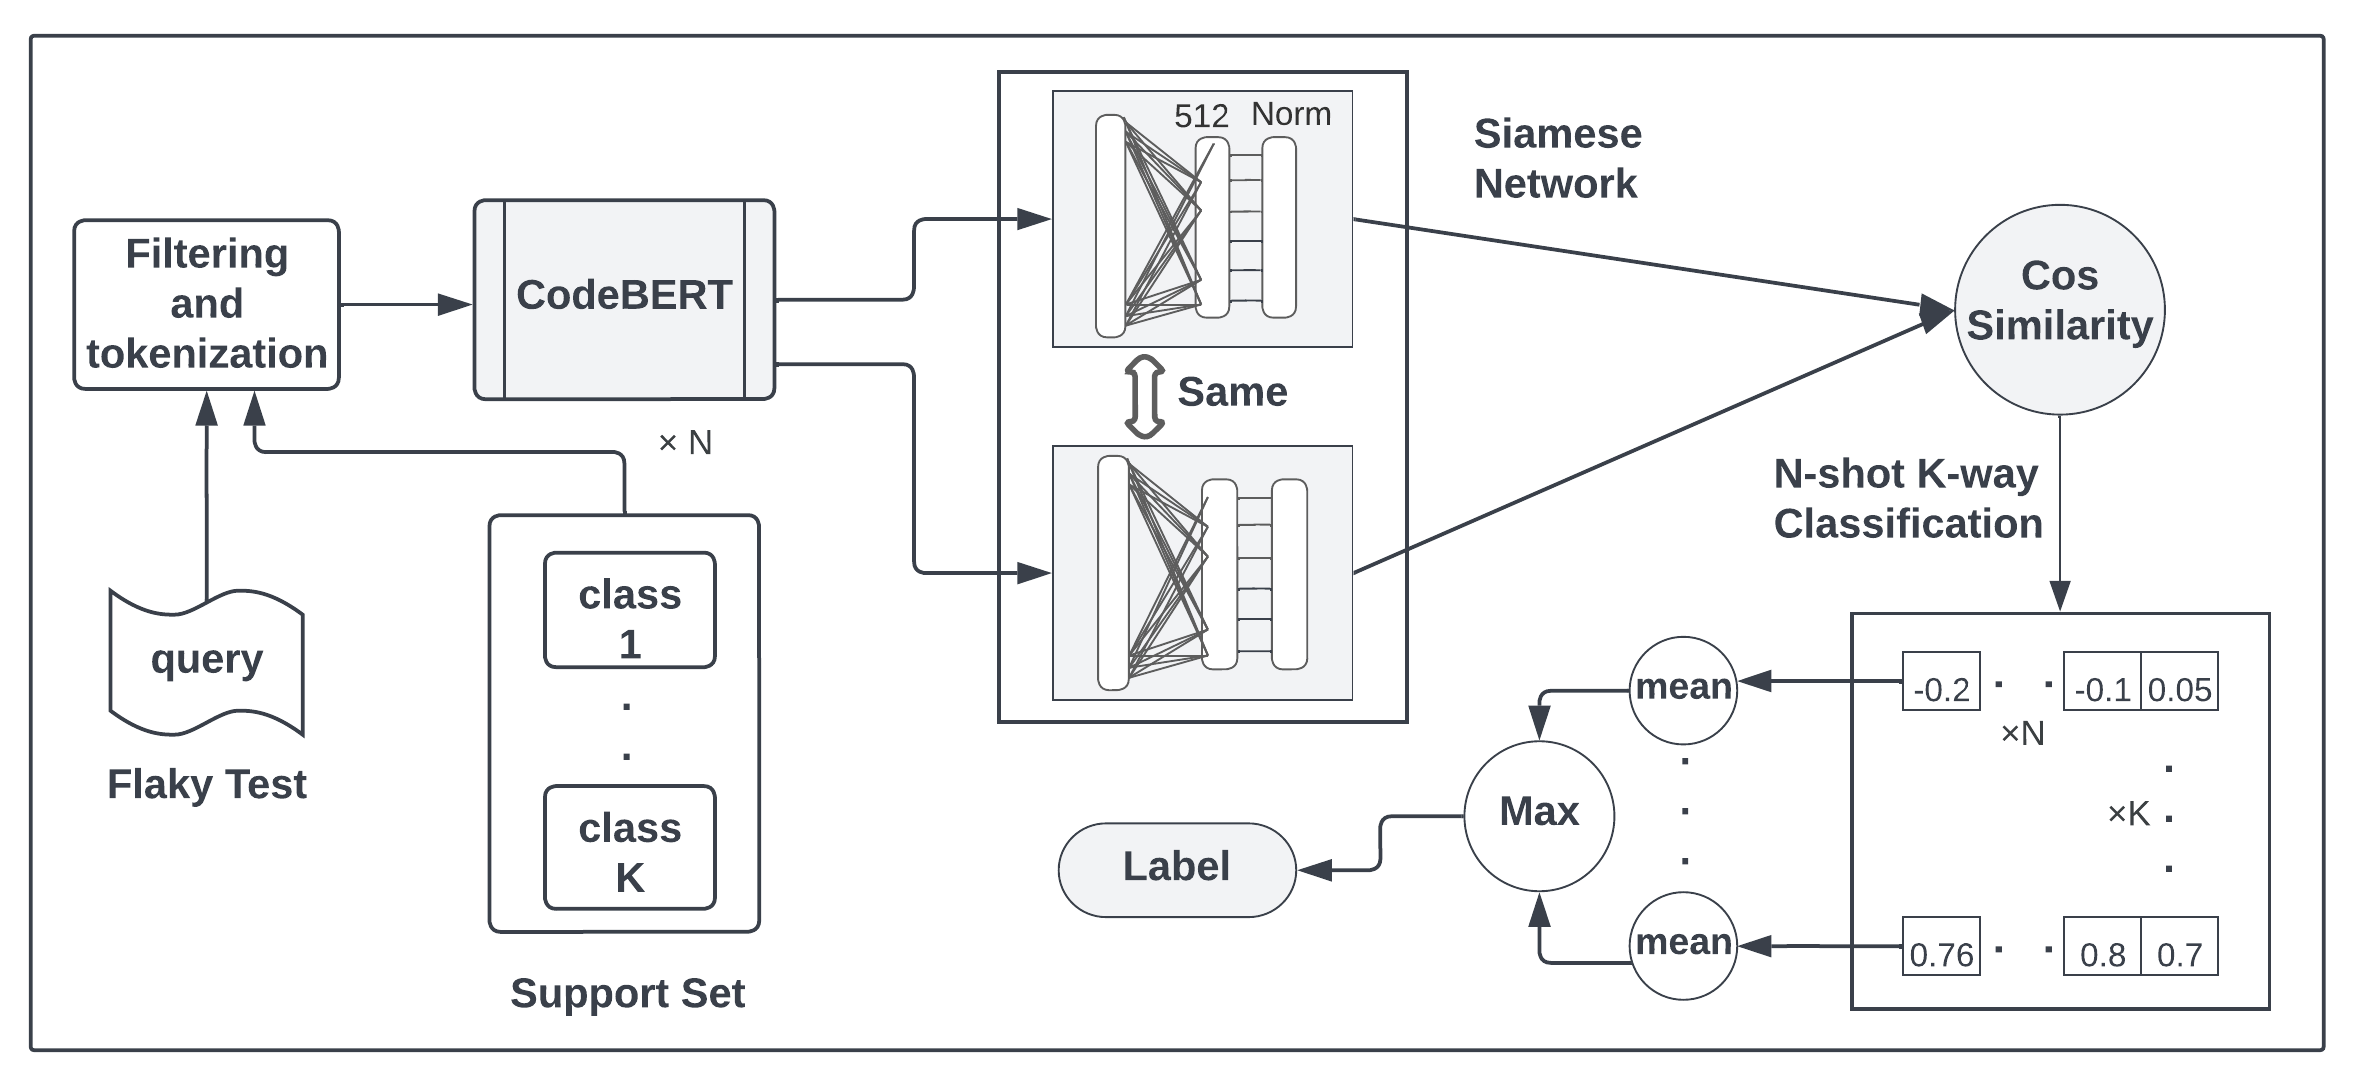
\includegraphics[width=0.8\textwidth,scale=1]{figures/flakycat/architecture.png}
\caption{An overview of FlakyCat, which combines the use of the pre-trained model CodeBERT, and Few Shot Learning based on the Siamese network.}
\label{fig:general_arch}
\end{figure}

In this section, we present the design and implementation of our approach.
Figure~\ref{fig:general_arch} presents an overview of the main steps of FlakyCat, code transformation and classification. 

\subsection{Step 1: Flaky test transformation}

\subsubsection{Scope} We rely on the test code to assign flaky tests to different categories.
Previous studies showed that flakiness finds its root causes in the test in more than 70\% of the cases\cite{Luo2014,Lam}. 
Hence, focusing on the test code allows us to capture the nature of flakiness while minimizing the overall cost of FlakyCat. 
Indeed, considering the code under test would require running the tests and collecting the coverage, which entails additional requirements and costs.



\subsubsection{Flaky test vectorization}
In order to perform a source code classification task, we first need to transform the code into a suitable representation that will be fed to the classification model. Among previous studies predicting flaky tests statically, two main approaches were used to transform code into vectors: using test smells~\cite{camara2021use,FlakeFlagger} and using code vocabulary \cite{pinto2020vocabulary,Haben2021,Camara2021VocabExtendedReplication}.
Both approaches seem promising, as different studies report high-performance models. As their encoding enables flaky test prediction, we believe they could also be used for flakiness category prediction, and we compare them with our approach. 


Recently, code embeddings from pre-trained language models were also considered for source code representation~\cite{fatima2021flakify,zhou2021assessing}. Pre-trained language models allow the encoding of code semantics and are intended for general-purpose tasks such as code completion, code search, and code summarization.
Considering these benefits, we use the pre-trained language model CodeBERT \cite{feng-etal-2020-codebert} to generate source code embeddings. 
CodeBERT can learn the syntax and semantics of the code and doesn't require any predefined features \cite{wan2022they}. Considering this aspect, we decide to rely on the CodeBERT test representation.

CodeBERT has been developed with a multi-layer transformer architecture~\cite{transformer} and trained on over six million pieces of code involving six programming languages (Java, Python, JavaScript, PHP, Ruby, and Go). 

To get the code representation using CodeBERT model, we first filter out extra spaces such as line breaks and tabs from the source code. In our case, we use each test method's source code as individual sequences. We then tokenise sequences by converting each token into IDs. Each sequence is passed to the CodeBERT model, which returns a vector representation. Figure~\ref{fig:using_codebert} illustrates this process.

Next, we explain the inputs and outputs of CodeBERT.

\paragraph{Inputs}
CodeBERT is able to process both source code and natural language, \eg comments and documentation. In our case, we did not exploit the possibility of using comments as the input length of CodeBERT is limited. Furthermore, comments can add noise since they represent unstructured text, possibly written by different developers, so we decided to solely rely on the code semantics. 
Hence, the given input to CodeBERT only considers code tokens, surrounded by two special tokens for boundaries. This is represented as follows: 
\begin{center}
 \([CLS], c1, c2, ..., cm, [SEP]. \)
\end{center}
Where \textit{Ci} is a sequence of code tokens, the special token [SEP] indicates the end of the sequence, and [CLS] is a special token placed in the beginning, whose final representation is considered as the representation of the whole sequence which we use for classification.


\paragraph{Outputs}

CodeBERT output includes two representations. The first one is the context matrix where each token is represented by a vector, and the second one is the CLS representation, having a size of 768, which is an aggregation of the context matrix and represents the whole sequence.
For the purpose of FlakyCat, we are interested in the CLS vector that represents the complete test code.

 
\begin{figure}[htbp]
\centering
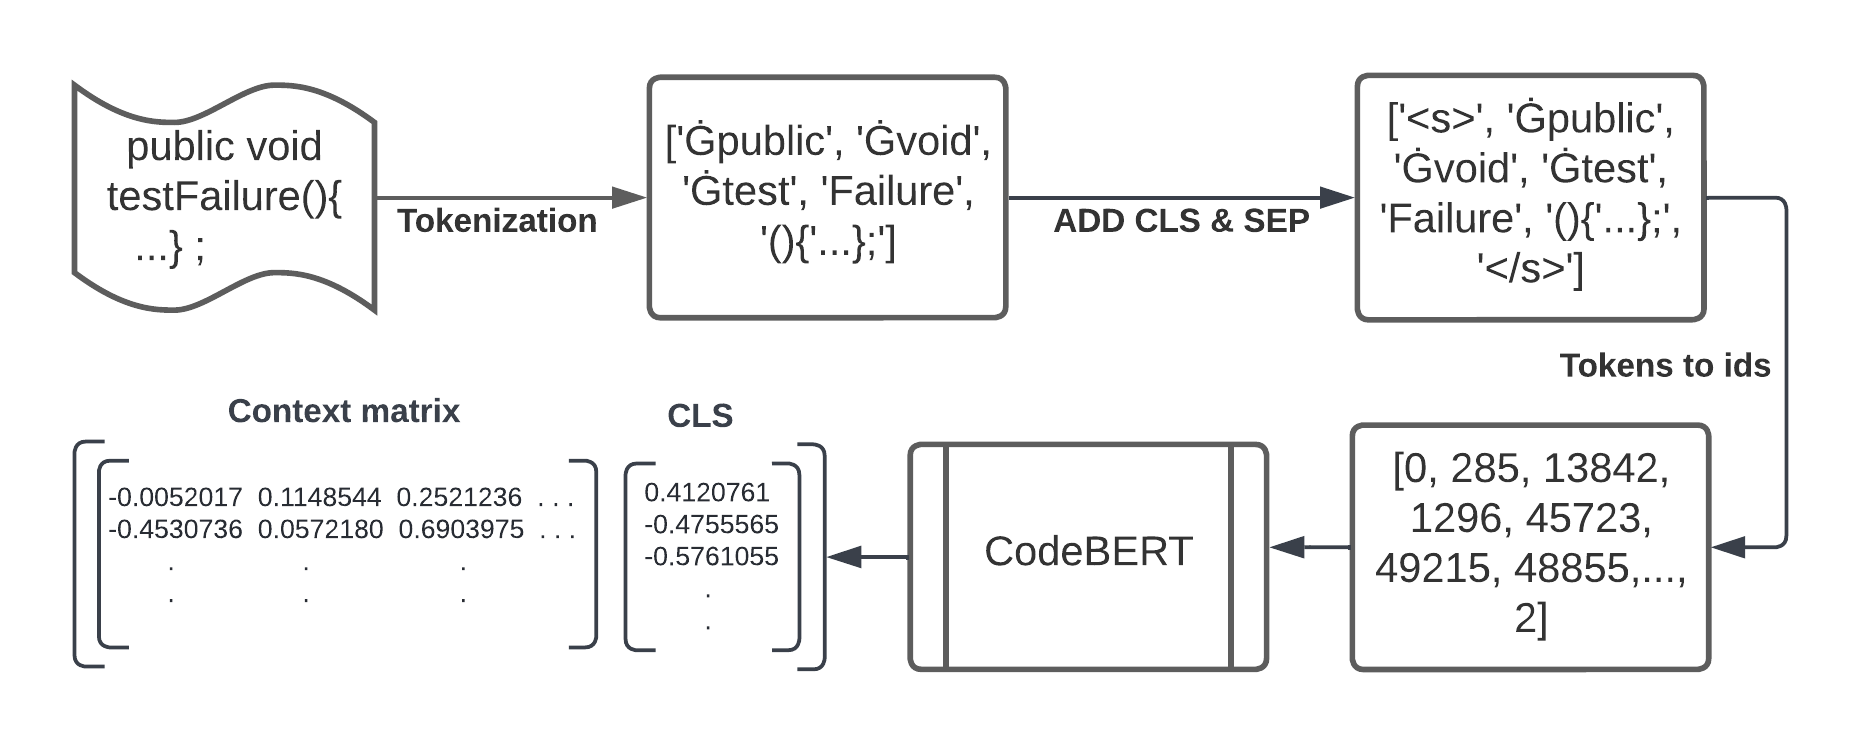
\includegraphics[width = 0.8\textwidth, scale=1]{figures/flakycat/codebert_transform.png}
\caption{The process of converting the source code of each test case to a vector using CodeBERT, going through tokenization, then converting to IDs and applying the CodeBERT model to get the representation (CLS vector). Ǵ represent spaces, $<s>$ used for CLS, and $</s>$ for SEP. }
\label{fig:using_codebert}
\end{figure}

\subsection{Step 2: Flaky test categorization}

\subsubsection{Classification process}

Unlike traditional machine learning classifiers that attempt to learn how to match an input $x$ to a probability $y$ by training the model in a large training dataset and then generalizing to unseen examples, Few-Shot Learning (FSL) classifiers learn what makes the elements similar or belonging to the same class from only a few data. Facing the scarcity of data on flaky tests, selecting an FSL classifier seems then to be a promising choice. 


In FSL, we call the item we want to classify a \textit{query}, and the \textit{support set} is a small set of data containing few examples for each class used to help the model to make classifications based on similarity as shown in Figure~\ref{fig:general_arch}.
To classify flaky tests according to their flakiness category, we compute the similarity between the query and all examples of each flakiness category in our Support Set and assign the label having the maximum similarity with the query. This classification is obviously performed in a space where all elements of the same class are similar or close to each other. This is achieved by a model called \textit{Siamese network}. Its task is to transform the data and project it into a space where all the elements of a same class are close to each other, and then to classify the elements by computing their similarity.



The Siamese network has knowledge of the similarity of elements of the same class. It processes two vectors in input and applies transformations that allow minimizing the distance between the two vectors if they share similar characteristics. Figure~\ref{fig:before_after} shows an example of the visualization of flaky test vectors before and after the Siamese network is applied. Since CodeBERT has no knowledge of the characteristics of flaky tests and only generates a general representation of the source code, the vectors produced are all similar.
However, the Siamese networks learn which characteristics in these vectors are shared by tests of the same class, and thus allow to project vectors into a space that groups tests of the same flakiness category. After this step, it becomes possible to classify them using a similarity computation.

\begin{figure}[htbp]
\centering
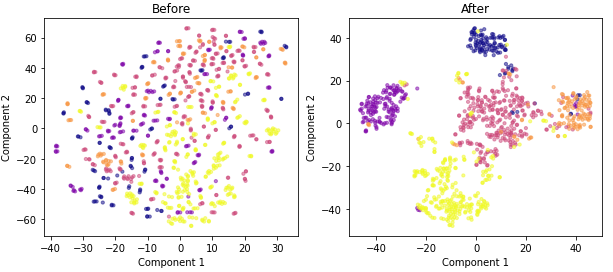
\includegraphics[width = 0.8\textwidth, scale=1]{figures/flakycat/before_after.PNG}
\caption{Visualization of our data before and after training of the Siamese network with the triplet loss, which brings together the elements of the same class.}
\label{fig:before_after}
\end{figure}
\vspace{3mm}

\subsubsection{Model training}


Siamese networks have two identical sub-networks, each sub-network processes the input vector and performs transformations.
Both sub-networks are trained by calculating the similarity between the two inputs and using the similarity difference as a loss function.
Accordingly, the weights are adjusted to have a high similarity if the inputs belong to the same class. For the architecture of the sub-networks, we used a dense layer of 512 neurons and a normalization layer as shown in Figure~\ref{fig:general_arch}.
We also performed a linear transformation to keep relations learnt by CodeBERT using the attention mechanism introduced in the transformer architecture \cite{attention}. 
This model is trained using a Triplet Loss function, based on the calculation of similarity difference.

Let the Anchor $A$ be the reference input (it can be any input), the positive example $P$ is an input that has the same class as the Anchor, the negative example $N$ is an input that has a different class than the Anchor, $s()$ is the cosine similarity function, and $m$ is a fixed margin. The idea behind the Triplet Loss function is that we maximize the similarity between $A$ and $P$, and minimize the similarity between $A$ and $N$, so ideally $s(A, P)$ is large and $s(A, N)$ is small. The formula for this loss function is: 

\vspace{3mm}
\begin{center}
\( Loss = max(s(A, N) - s(A, P) + m, 0) \)
\end{center}
\vspace{3mm}

$m$ is an additional margin as we do not want $s(A, P)$ to be very close to $s(A, N)$, which would lead to a zero loss. 

To train the Siamese network with the triplet loss, we give as input batches of pairs with the same classes, and any other pair of a different class can be used as a negative example. We select the closest negative example to the anchor, such as $s(A,  N)$ $\simeq$ $s(A, P)$, which generates the largest loss and constitutes a challenge for model learning. 
\section{Interpretability}
\label{sec:flakycat-interpretability}

% What is interpretability
Model interpretability refers to one's ability to interpret the decisions, recommendations, or in our case the predictions, of a model. Interpretability is a crucial step to increase trust in using a machine learning model. Indeed, it allows model creators to investigate potential biases in the learning processes and better assess the overall performance of their models.
On top of that, providing developers with information about how the model came to its prediction can enhance the model adoption~\cite{carvalho2019machine}. 

% Existing techniques
Flakiness prediction approaches often relied on Information Gain to explain what features in the model appeared to be the most useful~\cite{Pinto2020,FlakeFlagger,camara2021use}. In the case of tree-based models, the reported information gain is given by the Gini importance (also known as Mean Decrease in Impurity)~\cite{Featurei12:online}.
Parry \etal~\cite{flake16} used SHapley Additive explanations (SHAP), which is another popular technique for model interpretability~\cite{shaponline}. 

% Use of CodeBERT increasing
As FlakyCat uses the CodeBERT representation of tests as input, using the previously mentioned techniques would not give understandable features. To our knowledge, there are no existing techniques used for CodeBERT-based model interpretability. Thus, we introduce a novel approach to better understand the decisions of CodeBERT-based models. Following the main motivation of helping developers better understand flaky tests once detected, our goal with this interpretability technique is to arm FlakyCat users with a more fine-grained explanation for the model's decision.

% Our technique
Our technique is inspired by delta debugging algorithms. Delta debugging is used to minimize failure-inducing inputs to a smaller size that still induces the same failure~\cite{zeller2002simplifying}. In our case, we are interested in the particular code statements linked with the most influential information for the model's decision.
To identify them, we proceed with the following: We classify all the original test cases and save their similarity scores. We create new versions of each test. Each version is a copy of the original test minus one statement that was removed. 

Next, we feed the new versions to FlakyCat. Among all new versions for one test, we keep the one for which the similarity score endured the biggest drop compared to the original prediction score. 
We consider the statement removed in this version as the most influential one.
\section{Evaluation}
\label{sec:flakycat-evaluation}

In this section, we explain our evaluation setting for FlakyCat.
First, we describe our data curation process, then, we present our approach for answering each of the three research questions. 



\subsection{Data curation}
\label{dataset}

\subsubsection{Collection}
For our study, we had to collect a set of flaky tests containing their source code and their flakiness category.
We focused our collection efforts on one programming language, as training a classifier using code and tokens from different programming languages is more challenging. 
For the language choice, we opted for Java, which is the most common language in previous flakiness studies (and thus datasets). 
To increase the amount of data used in this study, we also collected a new set of flaky tests mined from GitHub that we classified manually.


\paragraph{Existing datasets} 

\begin{table}[htbp]
\centering
\caption{Data filtering performed on the different datasets used in this study. Collected represents the new dataset we retrieved.}
\begin{tabular}{|c|c|c|c|c|c|}
\hline 
\textbf{ Filters}&\multicolumn{5}{|c|}{\textbf{Datasets}} \\
\cline{2-6} 
\textbf{} &  \cite{Luo2014} & \cite{across_pr} & \cite{habchi2022made} & \cite{Shi2019iFix} & Collected \\
\hline 
\textbf{Inspected commits} & 201 & 170 & 40 & 101 & 270\\
\hline 
 Commit not found  & 12 & 12 & 4 & 3 & 3\\
\hline
 Duplicated commit & 0 & 2 & 0 & 0 & 3 \\
\hline 
 Open commit & 0 & 0 & 0 & 33 & 0 \\
\hline
Flaky test not found & 45 & 21 & 13 & 0 & 42 \\
\hline 
Configuration problems & 3 & 8 & 0 & 0 & 0\\
\hline
Not Java & 15 & 5 & 0 & 0 & 8 \\
\hline 
Category hard to classify & 40 & 57 & 4 & 0 & 22 \\
\hline 
\textbf{Considered commits} & 86 & 65 & 19 &  65 & 192\\
\hline 
\rowcolor{Gray}
Total of extracted tests & 109 & 65 & 20  & 65 & 192\\
\hline
\end{tabular}
\label{tab:filtring_datasets}
\end{table}
\vspace{3mm}


There is no large public dataset of flaky tests labelled according to their category of flakiness. Most of the existing studies, such as FlakeFlagger~\cite{FlakeFlagger} and DeFlaker~\cite{deflaker}, are limited to list detected flaky tests which are later used for binary classification. 
%There is also the Illinois' dataset\footnote{https://mir.cs.illinois.edu/flakytests/}, which is partially classified into order-dependent and implementation-dependent flaky tests. 
Regarding the data classified into flakiness categories defined by Luo~\etal \cite{Luo2014} and Eck~\etal~\cite{eck}, there is only limited data available in previous empirical studies about flakiness. We retrieved tests from the empirical study of flaky tests across programming languages of Costa \etal~\cite{across_pr} and from a recent study about pinpointing causes of flakiness by Habchi \etal~\cite{habchi2022made}. We also retrieved the flaky tests from iFixFlakies~\cite{Shi2019iFix} as \textit{Test order dependency} is a flakiness category that received a large interest in the community~\cite{li2022evolution,Lam2019iDFlakies,li2022repairing,parry2022evaluating}.


We gathered a total of 512 commits/pull requests from the existing datasets we could access, referenced in Table \ref{tab:filtring_datasets}.

\paragraph{New dataset}
To expand existing datasets, we explore GitHub projects and search for flakiness-fixing commits for which developers explained the reason (\ie category) of flakiness.

In this search, we use flakiness-related keywords such as \textit{Flaky} and \textit{Intermit} in the commit messages. 
To ensure that the commit refers to a flakiness category, 
we further filter commits by specific keywords related to each category: \textit{thread, concurrence, deadlock, race condition} for Concurrency, \textit{time, hour, seconds, date format, local date} for Time, \textit{port, server, network, http, socket} for Network and \textit{rand} for Random.
After the search, we rely on the developer's explanation in the commit message and on the provided fix to classify tests into the different flakiness categories listed in the literature.
This collection allowed us to obtain 270 commits fixing flaky tests to be classified manually. 

\subsubsection{Filtering}
The previous step allowed us to collect a total of 782 categorized commits/issues. 
In this step, we filter out commits and data that are not adequate for our study. We filter out commits hard to classify, duplicated ones, and those where flaky tests are not written in java. Costa et al. \cite{across_pr} classified issues, and Luo et al. \cite{Luo2014} classified old SVN revisions. In some cases, the corresponding commit could no longer be found in the projects. Some data points were missing necessary attributes, such as the name of the flaky test. Particularly, in commits where the fix is in the production code or in a configuration file, and the test name of the involved flaky test is not indicated in the commit message, we were not able to identify the flaky test, so we filtered them out.
The number of tests extracted for each dataset is shown in Table \ref{tab:filtring_datasets}. The \textit{considered commits} row accounts for commits where all information needed was present \ie the test name, source and category of flakiness. Note that the number of considered commits and extracted tests vary in some cases as developers sometimes addressed more than one flaky test per commit.
We obtained a total of 259 flaky tests after filtering the existing datasets.
For the data we collected ourselves, we successfully extracted 192 test cases. To ensure the correctness of our manual classification and filtering, the first two authors of the paper performed a double-check on the newly collected dataset. 

\subsubsection{Processing}
After filling in all the necessary attributes: the test case name, flakiness category, test file name, and project URL, we download the code files and extract test methods using the spoon library\footnote{https://github.com/INRIA/spoon}. At this stage, all comments have been deleted from the source code to restrict CodeBERT to code statements.

\subsubsection{Final dataset}

The final dataset contains 451 flaky tests distributed over 13 flakiness categories.
Table~\ref{tabData} illustrates this distribution.

The collected flaky tests are not distributed evenly across categories of flakiness. Just as shown in past empirical studies~\cite{Luo2014,Gruber2021}, some categories, such as \textit{Async waits}, are more prevalent than others. 
Our approach uses FSL to learn from limited datasets. 
Still, it requires a certain amount of examples to learn common patterns from each category. 
We decided to have at least 30 tests in a category to consider it. This number is commonly accepted by statisticians as a threshold to have representativeness~\cite{why30}, since learning from very few examples is not feasible. In our dataset, some flakiness categories contain no more than 5 flaky tests. We were not able to gather more data for those non-prevalent categories and thus decided to focus on five of the most common flakiness categories, highlighted in grey in the table: \textit{Async waits}, \textit{Test order dependency}, \textit{Unordered collections}, \textit{Concurrency}, and \textit{Time}.


\subsubsection{Data augmentation}
Facing the challenge of learning from few data, we over-sampled our training set similarly to SMOTE~\cite{chawla2002smote} by applying elementary perturbations. In the same way, as we increase the imagery data by rotating and resizing, for the source code, we generate variants of our tests by mutating only the code elements that have no influence on flakiness. This includes variable names, constants such as strings, test method names, and by adding declarations of unused variables. In this way, the model will learn useful code elements instead of learning from variable names and strings. We used the Spoon library for the detection of these elements, and we replaced them with randomly generated significant words. As a result, the total number of tests after data augmentation is 964. 


\begin{table}[htbp]
\centering
\caption{Final dataset. The Highlighted rows are the data used to train and test the model. The original data refers to the data we collected, short data are tests with less than 512 tokens, and the augmented data are the data we obtained after augmentation. }
\begin{tabular}{|c|c|c|c|}
\hline
\textbf{Class}&\multicolumn{3}{|c|}{\textbf{Data}} \\
\cline{2-4} 
\textbf{} & \textbf{\textit{Original}}& 
\textbf{\textit{Short}} &
\textbf{\textit{Augmented}}  \\
\hline
	
\rowcolor{Gray}
Async waits & 125 & 97 &  300\\
\hline
\rowcolor{Gray}
Test order dependency & 103 & 100 &  284\\ 
\hline
\rowcolor{Gray}
Unordered collections & 51 & 48 & 146 \\
\hline
\rowcolor{Gray}
Concurrency & 48 & 40 & 124 \\
\hline
\rowcolor{Gray}
Time & 42 & 38 & 110 \\
\hline
Network & 31 & 25 & /\\
\hline
Randomness & 17 & 14 &  / \\
\hline
Test case timeout & 14 & 9 &  / \\
\hline 
Resource leak & 10 & 7 &  / \\
\hline
Platform dependency & 2 & 2 &  / \\
\hline 
Too restrictive range & 3 & 2 & / \\
\hline 
I/O & 2 & 2 & / \\
\hline 
Floating point operations & 3 & 1 & /\\
\hline

TOTAL & 451 & 385 &  964 \\
\hline
\end{tabular}
\label{tabData}
\end{table}
\vspace{1mm}


\subsection{Experimental design}
\subsubsection{Baseline}
~~ \\
To the best of our knowledge, we are the first to introduce an automatic classification of flaky tests according to their category.
However, to get a better appreciation of the performance of the solution we propose in this paper, we seek to compare FlakyCat with test representations commonly used by flaky test detection approaches. Our intuition is that test representations giving good performance in binary classification (\ie detecting flaky tests and non-flaky tests) have a good chance to be helpful for the classification of tests according to their category of flakiness. Thus, we use the following representations for our multi-classification task: the vocabulary-based approach \cite{pinto2020vocabulary} which is a keyword-based approach, and the smell-based approach \cite{camara2021use} which exploits the correlation between test smells and test flakiness. Our overall motivation is to determine whether it is possible to make this classification based on limited data and to know which combination of classifier and code representation delivers the best results. 

For the classification based on test smells, we use the 21 smells detected by tsDetect \cite{tsdetect}, to generate vectors indicating the presence of each smell detected by the tool, in the same way as in the study of Camara \etal \cite{camara2021use}. As for the vocabulary-based classification, we use token occurrence vectors, as in the article by Pinto \etal \cite{pinto2020vocabulary}. We tokenize the code and apply standard pre-processing like stemming, then calculate occurrences of each token.

In addition to various test representations, we compare our FSL-based approach with traditional classifiers from the Scikit-learn library~\cite{pedregosa2011scikit} used by previous studies on flakiness prediction~\cite{pinto2020vocabulary,camara2021use,Camara2021VocabExtendedReplication}: Random Forest (RF), Support Vector Machine (SVM), Decision Tree (DT) and K-Nearest Neighbour (KNN). 

% We also compare the code representation used in our classification approach with the different source code representations used in the context of flaky tests, in particular, vocabulary vectors, which is the primary tokens-based method used to represent text and its semantics in machine learning tasks, including source code classification. The second is the test smells representation, based on vectors indicating the presence of certain test smells that may have a relation with test flakiness according to previous studies \cite{FlakeFlagger,camara2021use}.




To validate each model, we split our data into 75\% for training and 25\% for final validation. We use a 10-fold stratified cross-validation on the training data to select the best model parameters and use those parameters to evaluate the model on the unseen hold-out set.

As the augmented samples in our dataset are variants of the original ones, it was important to keep them in the same sets, to ensure that no similar data pairs are included in both the training and test sets. For the support set used for classification, we select the most centred examples to represent each class. 

FlakyCat relies on a Siamese network. It is trained with combinations of data by indicating whether these data are similar or not so that the model can learn what makes them similar. Since we train with combined data, the balancing of data is not required, because it is automatically over-sampled.



\subsubsection{Parameters}
~~ \\
We tuned FlakyCat's parameters on the training set using the Random Search method~\cite{bergstra2012random} and a 10-fold cross-validation, by testing random combinations of the most important parameters that have a direct impact on the model performance, which include the similarity margin used in the triplet loss function, the learning rate, the number of warm-up steps, and the support set size.

Figure ~\ref{fig:parameters} shows the resulting weighted F1 score for each tested parameter combination using a 10-folds cross-validation. A high learning rate and a number of warm-up steps have a negative impact on the performances, while other parameters have a lower influence.  Following these results, for the final validation on the hold-out set, we use the best parameter combination identified in the Figure~\ref{fig:parameters}: a similarity margin of 0.30, a learning rate of 0.001, a number of warm-up steps of 400, and a support set with 10 examples from each category.

For baseline classifiers, we keep the standard values used by previous works. We varied the number of trees in the Random Forest classifier, we tested values from 100 to 1000 with a step of 100.
We observed that this does not make much difference regarding the F1 score ($\leq$ 3\%), and we identified 1000 as the number giving the best results. 


\begin{figure}[htbp]
\centering
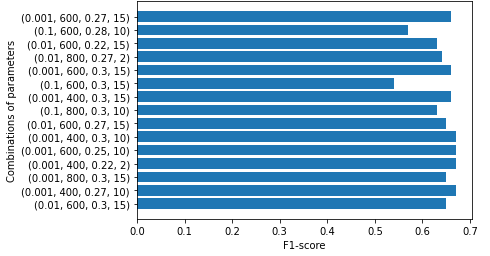
\includegraphics[scale=0.7]{figures/flakycat/parameters.PNG}
\caption{F1 score for different values of parameter combinations using Random Search and a 10-Folds cross-validation. The combinations on the Y axis have the form : (learning rate, number of warm-up steps, similarity margin, support set size). }
\label{fig:parameters}
\end{figure}



\subsubsection{Evaluation metrics}
~~ \\
We use the standard evaluation metrics to compare classifiers, including precision, recall, Matthews correlation coefficient (MCC), F1 score, and Area under the ROC curve (AUC).
These metrics have been used to evaluate the performance of classifiers, including binary classification of flaky tests~\cite{pinto2020vocabulary,camara2021use,fatima2021flakify}.
Since our dataset is unbalanced, weighted metrics are more suitable for our evaluation. 


\subsubsection{Research questions}
\paragraph{  \textbf {RQ1: How effective is FlakyCat compared to approaches based on other combinations of test representation and classifier?}}

This question aims to evaluate FlakyCat and compare it to other test representation techniques, \ie vocabulary and test-smell-based and traditional classifiers, \ie SVM, KNN, decision tree and random forest.

\paragraph{  \textbf {RQ2: How effective is FlakyCat in predicting each of the considered flakiness categories?}}

This question evaluates FlakyCat's ability to classify the different categories of flakiness.
To perform this, we split the dataset into five sets following the categories: \textit{Async waits}, \textit{Test order dependency},  \textit{Unordered collections}, \textit{Concurrency}, and \textit{Time}.
Then, we use the same settings as for RQ1 to tune the Siamese network, train it, and evaluate it for each category.

\paragraph{  \textbf {RQ3: How do statements of the test code influence the predictions of FlakyCat?}}

We applied the technique we introduced in Section~\ref{sec:flakycat-interpretability} for CodeBERT-based model interpretability to FlakyCat. 
We classified all original short data (323 tests). For 16 tests, the score doesn't decrease by deleting one statement, and thus we collected 307 statements of interest, important for FlakyCat's decision-making.
%We collected the most influential statement for each flaky test classified correctly. 
To better understand what information emerges, we proceeded with the following analysis. First, we regroup statements by category of flakiness (according to the flaky test they belong to). Then, we want to share information on what type of statements FlakyCat found useful. To do so, we look through the list of statements and attempt to identify recurring code statements and categorize them. The process of identifying statement types is exploratory and inspired by qualitative research. Two of the authors of this paper went through the list of statements and identified nine recurring types of statements:
\begin{itemize}
 \item \textbf{Control flow:} Includes decision-making statements, looping statements, branching statements, Exception handling statements.
 \item \textbf{Asserts:} All types of assertions in tests. 
 \item \textbf{Threads:} statements related to threads and runnables. 
 \item \textbf{Constants:} Constant values such as strings, numbers and boolean values independent of variables, and final variables. 
 \item \textbf{Waits:} All explicit wait statements. 
 \item \textbf{Usage of date/time:} Statements that perform operations on time values, dates. 
 \item \textbf{Network:} Statements related to data exchange in a local or external network between two endpoints, and session management. 
 \item \textbf{I/O:} Statements related to input/output, database and file access. 
 \item \textbf{Global variables:} Includes the use of global variables. 
\end{itemize}

With this question, we investigate the prevalence of these statement types in each flakiness category.
\section{Results}
\label{sec:flakycat-resuts}

\subsection{RQ1: How effective is FlakyCat compared to approaches based on other combination of test representation and classifier? } 

\begin{table*}[htbp]
\caption{Comparing performances of FlakyCat (CodeBERT and Few-Shot Learning) with traditional machine learning classifiers}
\centering
\begin{tabular}{|c|c|c|c|c|c|c|c|c|c|c|c|c|c|c|c|}
\hline
\textbf{Model} & \multicolumn{5}{|c|}{\textbf{Smells-based}} & \multicolumn{5}{|c|}{\textbf{Vocabulary-based}} &\multicolumn{5}{|c|}{\textbf{CodeBERT-based}} \\
\cline{2-16} 
\textbf{} & \textbf{\textit{Precision}}& \textbf{\textit{Recall}} & \textbf{\textit{ MCC}}& \textbf{\textit{F1}} & \textbf{\textit{AUC}}& \textbf{\textit{Precision}}& \textbf{\textit{Recall}} & \textbf{\textit{ MCC}}& \textbf{\textit{F1}} & \textbf{\textit{AUC}} & \textbf{\textit{Precision}}& \textbf{\textit{Recall}} &\textbf{\textit{ MCC}}& \textbf{\textit{F1}} & \textbf{\textit{AUC}}\\
\hline


SVM & 0.11 & 0.34 & 0.00 & 0.17 & 0.50
& 0.61 & 0.52 & 0.37 & 0.45 & 0.66 
& 0.27 & 0.43 & 0.22 & 0.33 & 0.60 \\

\hline

KNN & 0.24 & 0.37 & 0.11 & 0.29 & 0.55
& 0.44 & 0.48 & 0.31 & 0.45 & 0.65 
& 0.56 & 0.53 & 0.37 & 0.51 & 0.68 \\

\hline

DT & 0.31 & 0.33 & 0.10 & 0.23 & 0.53 
& 0.53 & 0.53 & 0.39 & 0.52 & 0.69
& 0.49 & 0.50 & 0.34 & 0.49 & 0.67 \\

\hline

RF & 0.32 & 0.34 & 0.12 & 0.24 & 0.54
& 0.72 & 0.61 & 0.49 & 0.56 & 0.72 
& 0.68 & 0.66 & 0.55 & 0.62 & 0.76 \\

\hline
\textbf{FSL} & 0.13 & 0.18 & -0.01 & 0.13 & 0.50 
& 0.69 & 0.68 & 0.58 & 0.67 & 0.79
& \textbf{0.74} &\textbf{0.73} & \textbf{0.65} & \textbf{0.73} & \textbf{0.83} \\
\hline
\end{tabular}
\label{scores}
\vspace{-5mm}
\end{table*}

Following the outlined experimental design, we trained and tested FlakyCat and the four traditional classifiers, using the three source code representations, the vectors obtained from CodeBERT, the vectors based on vocabulary, and the ones based on test smells. The obtained results are presented in Table~\ref{scores}. The results show that FlakyCat achieves the best performance for all evaluation metrics. 
It obtained an average weighted F1 score of 73\% and a precision of 74\%.
We get an MCC of 0.65 (bounds for this metric are between -1 and 1), being close to 1 means a perfect classification. Finally, the AUC of 0.83 shows that the model is able to distinguish flaky tests from different classes. 

\paragraph{Representation effect}
Regarding the three code representations, CodeBERT achieves the best performance for RF, KNN, and FSL, with an F1 score between 0.51 and 0.73 for the three classifiers. 
When using the vocabulary-based vectors, SVM and DT perform better than using CodeBERT. With this representation, all classifiers do not exceed an F1 score of 0.67.
The representation based on test smells yields lower results, with the best F1 score being 0.29.
The CodeBERT representation seems then promising to use when learning to classify flaky tests according to their categories. 

\paragraph{Classifier effect}
Regarding the choice of classifier, we find that the FSL classifier based on similarity achieves the best performance using the representations based on CodeBERT and vocabulary. Among traditional classifiers, Random Forest obtains the best results, as reported in previous flaky test classification studies~\cite{Pinto2020,Haben2021}. Classifiers relying on the smell-based representation have more difficulty to classify flaky tests. Using this code representation, the KNN classifier achieved the best F1 score: 0.29. Two categories had a positive impact to achieve this score: \textit{Async wait}, and \textit{Test order dependency}. This can be explained by the presence of test smells strongly related to these two categories, including Sleepy test and Resource optimism. Other flakiness categories seem to be more challenging to predict using existing test smells. 

\paragraph{Random-guessing comparison}
In the previous paragraph, we compared different models and different code representations and saw that FlakyCat gave the best results. Because all the existing approaches were designed to detect flaky tests from non-flaky tests, they might not be suitable for the specific task of classifying flaky tests according to their categories. As no other category-based classification technique exist so far, we show the performance of a random guesser as another baseline. We consider two random guessing approaches, the first one where we randomly affect a class to each flaky test and the second one where we weigh the random affectation according to the prevalence of flaky tests in each category. Both approaches are considered as the dataset balance might be different from the one found in various projects. Results are listed in Table ~\ref{scores-random}. F1 scores for Random and Weighted Random are respectively of 0.21 and 0.25. With an F1 score of 0.73, we see that FlakyCat performs better than the two considered random-guessing approaches. 

\begin{tcolorbox}

\textbf{RQ1} Overall, our results show that automatic classification of flaky test categories with a limited amount of data is a challenging but feasible and promising task. 
% it is possible to automatically classify flaky test categories with a limited amount of data. 
The representation based on CodeBERT gives better results compared to the ones based on test smells and vocabulary. We also found that Few Shot Learning performs better than traditional machine learning classifiers. 

\end{tcolorbox}

\begin{table}[ht]
\caption{Performance of random guessing approach}
\centering
\begin{tabular}{|c|c|c|c|c|c|}
\hline
\textbf{Method} & \textbf{\textit{Precision}}& \textbf{\textit{Recall}} & \textbf{\textit{ MCC}}& \textbf{\textit{F1}} & \textbf{\textit{AUC}} \\
\hline
Random & 0.25 & 0.20 & -0.01 & 0.21 & 0.50 \\
\hline
Weighted Random & 0.25 & 0.26 & 0.02 & 0.25 & 0.51 \\
\hline
\end{tabular}
\label{scores-random}
\end{table}

\subsection{RQ2: How effective is FlakyCat in predicting each of the considered flakiness categories?}

\begin{figure}[htbp]
\centering
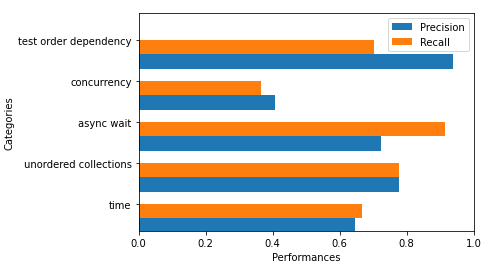
\includegraphics[scale=0.8]{figures/flakycat/FSL.PNG}
\caption{Precision and Recall per flakiness category using FlakyCat}
\label{fig:FSL}
\end{figure}

Figure~\ref{fig:FSL} shows performances achieved by FlakyCat for each of the five flakiness categories. Results show that the category \textit{Async wait} is the easiest for the model to classify, with an F1 score of 0.81. The category \textit{Test order dependency}, \textit{Unordered collections} and \textit{Time} respectively have an F1 score of 0.80, 0.78 and 0.66. \textit{Concurrency} performances are lower with an F1 score of 0.39. 
We suspect that concurrency issues happen in many cases in the code under test. As FlakyCat only relies on the test source code, this would indeed explain why performances are lower in this case. Another supposition is that concurrency issues and asynchronous waits are sometimes closely related. We discuss an example of this in Section~\ref{sec:discussion:reasoning}. \\




%\begin{table}[htbp]
%\caption{Performances by categories using FlakyCat}
%\begin{center}
%\begin{tabular}{|c|c|c|c|}
%\hline

% the scores avg for the cross validation 

%\textbf{Category} & \textbf{\textit{Precision}}& \textbf{\textit{ Recall}} & \textbf{\textit{Weighted F1-score}} \\
%\hline
%Unordered collections & 0.78 & 0.78 & 0.78 \\
%\hline
%test order dependency & 0.94 & 0.70 & 0.80 \\
%\hline
%Async waits & 0.72 & 0.92 & 0.81 \\
%\hline
%Time & 0.65 & 0.67 & 0.66 \\
%\hline
%Concurrency & 0.41 & 0.37 & 0.39 \\
%\hline
%\end{tabular}
%\label{tab_classes}
%\end{center}
%\end{table}

\begin{tcolorbox}

\textbf{RQ2} While the four flakiness categories \textit{Async waits}, \textit{Test order dependency}, \textit{Unordered collections},  and \textit{Time} show good ability to be detected automatically, \textit{Concurrency} remains difficult to detect by relying only on the test case code. 

\end{tcolorbox}

\begin{table*}[htbp]
\caption{Prevalence of different types of statements in each flakiness category for true positive predictions }
\centering
\resizebox{\textwidth}{!}{
\begin{tabular}{|c|c|c|c|c|c|c|c|c|c|c|}
\hline
 & \#Statements &	Control flow &	Constants &	Asserts &	Threads	& Waits &	Network & Global variables &	Usage of Date/time	 & I/O \\
\hline 
Async Waits & 80 &	16,25\% &	55\%   &	20\%	& 20\% &	27,5\% &	25\% &	11,25\% & 	3,75\% & 	6,25\% \\

\hline 
Concurrency & 34 &	23,53\% &	47,06\% &	17,65\% &	29,41\% &	14,70\% &	14,70\% &	5,88\% &	17,65\% & 2,94\%  \\
\hline 

Test order dependency & 69 &	8,69\% &	60,87\% &	13,04\% & 0\% &	4,35\% &	8,69\% &	2,90\% &	7,25\% &	47,82\% \\

\hline 

Time & 32 &	18,75\% &	56,25\% &	50\%	& 0\%	& 0\% & 	0\% &	9,375\% &	62,5\% &	6,25\% \\
\hline 

Unordered collections & 42 &	4,76\% &	66,67\% &	38,09\% &	0\% &	0\% &	2,38\% &	4,76\% &	0\% & 4,76\%  \\
\hline
\end{tabular}
}
\label{TabStatments}
\vspace{-5mm}
\end{table*}

\subsection{RQ3: How do statements of the test code influence the
predictions of FlakyCat?}

Table~\ref{TabStatments} reports the prevalence (\%) of the different types of statements among all influential statements per flakiness category, \eg 100\% Asserts in the \textit{Time} category would mean that all influential statements for the \textit{Time} category contain assert statements. 

Compared to other flakiness categories, the percentage of assertions in the influential statements of \textit{Time} and \textit{Unordered collections} is high, 50\% and 38.09\% respectively. Based on our analysis, this includes in particular assertions that perform exact comparisons, such as \texttt{assertEquals()}, between constant values and collection items, or dates for example. 
29,41\% of influential statements in the \textit{Concurrency} category include thread manipulation, and 20\% for the \textit{Async Waits} category, while the rest of the categories have none. 
Statements containing explicit waits represent respectively 27,5\% and 14,7\% for \textit{Async Waits} and \textit{Concurrency} categories, but below 5\% for \textit{Test order dependency} and zero for the others. Statements containing date or time values are most common in the \textit{Time} category with 62,5\%. We note that they appear as well in a small proportion, 17,65\%, for \textit{Concurrency}. Statements from the I/O calls group are mainly found in the \textit{Test order dependency}.
For \textit{Control flow}, \textit{Constants}, and \textit{Global variables} statements are almost evenly distributed. We include a spreadsheet containing all statements analyzed in our replication package. 

% The results show that FlakyCat is able to differentiate between the features that are important to each flakiness category by considering the correlation between the types of statements and flakiness categories. This also suggests that CodeBERT is able to grasp some semantics from the test code. \\

\vspace{2mm}
\begin{tcolorbox}
\textbf{RQ3} The interpretability technique we presented enable us to find which statements impact FlakyCat's decision. We also find hints that specific flakiness categories have distinct statement types (\eg Usage of Date/time for the \textit{Time} category) while some others have similar prevalence (\eg Threads for \textit{Async Waits} and \textit{Concurrency} categories).
By highlighting these statements, our interpretability technique may provide information to developers to better understand flaky tests, their categories and their causes.
\end{tcolorbox}

% asserts -> Time & unordered collections
% New instance & constants -> same distribution across categories
% time -> mostly time but also async waits and concurrency ( not for collections )
% threads & waits -> only async waits and concurrency
% external API calls -> mainly Async waits & concurrency

% 1. model learnt what needs to be learnt and Codebert learns good features 
% 2. 


\section{Discussion}
\label{sec:flakycat-discussion}

\subsection{Reasoning about the statements influencing FlakyCat and the usage of flakiness categories}
\label{sec:discussion:reasoning}

Listing~\ref{lst:flaky-example} gives an example of a flaky test taken from the Neo4J project\footnote{https://github.com/neo4j/neo4j/commit/c77e579b40b02087} found during the data collection part.
As explained in the commit message, the flakiness was caused by a race condition and thus, we affected it to the Concurrency category. FlakyCat classified this test as Async wait. The interpretability technique that we introduced in Section~\ref{sec:flakycat-interpretability} reveals that the statement on line 6 is the most influential for the model's decision. It contains the \texttt{await()} function, and this is likely the reason why the flaky test was categorized as Async wait. Furthermore, similarity score for the Concurrency category is high, and it comes as FlakyCat's second guess. 

When looking at the test, we understand that an asynchronous wait was performed to wait for a thread. We also found similar examples concerning other categories, such as waits relying on network resources. First, we argue that our interpretability technique can help to understand the cause of flakiness, even when FlakyCat apparently mislabelled the test. Secondly, we advance that flakiness categories as commonly defined in research studies~\cite{Luo2014, Eck2019} can overlap, \ie a flaky test can belong to several categories. The application of machine learning to determine the causes of flakiness is promising and should receive attention. It would also benefit from a more precise, orthogonal classification of flakiness categories. \\


\begin{lstlisting}[caption={A flaky test belonging to two categories
},label={lst:flaky-example},language=Java]
@Test
public void shouldPickANewServer[...]() throws Throwable {
[...]
    Thread thread = new Thread( () -> {
    try {
    startTheLeaderSwitching.await();
    CoreClusterMember theLeader = cluster.
        awaitLeader();
    switchLeader( theLeader );
    } catch ( TimeoutException | InterruptedException e ) {
        // ignore
    }});
[...]
}
\end{lstlisting}

\subsection{The effect of considering an additional category}
Our results showed that flakiness categories can be classified automatically. We carried out our main experiments with five categories of flakiness for which we had a reasonable number of tests. Still, we believe that one interesting aspect of our study is to understand the impact of adding other categories to FlakyCat. 
For this, we investigate the performance of FlakyCat for each category (similarly to RQ2), but we add to our set the \textit{Network} category,
which is the next category with the most samples in our dataset (25 tests). F1 scores and the accuracy obtained for each category are presented in Figure \ref{fig:fsl_add_class}. 

Compared to the results previously reported in Table~\ref{scores}, we observe that the performances of each category are slightly impacted.
The \textit{Async waits} category is the most impacted one. 
Indeed, after adding the \textit{Network} category, we get an overall F1 score of 0.68. The added category gets the worst results. 
This performance drop can be explained by multiple factors.
First, having more categories to differentiate makes it more challenging for FlakyCat to distinguish between them.
Secondly, the overall F1 score is strongly affected by the poor performance observed in the new category.
The performance for the Network category can be a result of the too low number of examples in this category (25). Despite using FSL, the model still requires enough data points in each category. While collecting data, we noticed that flaky tests caused by Network were not common. These findings align with the ones about the prevalence of the different categories reported in previous empirical studies~\cite{Luo2014,Eck2019}. In addition, flaky tests related to \textit{Network} issues could also be considered as Asynchronous waits in many cases, as previously explained. 


\begin{figure}[htbp]
\centering
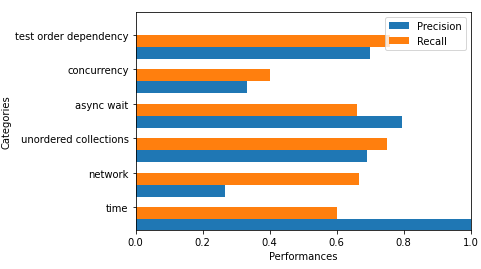
\includegraphics[scale=0.8]{figures/flakycat/add_network.PNG}
\caption{Precision and Recall per flakiness category when adding the category "Network" }
\label{fig:fsl_add_class}
\end{figure}
\section{Threats to Validity}
\label{sec:flakycat-threats}

\subsection{Internal Validity}
One threat to the internal validity is related to the dataset we used in our study. Flaky tests were gathered from different sources, as explained in Section~\ref{dataset}. It is possible that flaky tests were assigned to the wrong label, which would impact the training and evaluation of our model. Certifying the category based on the test source code is complex and can as well be subjective. To ensure the quality of the data, the first two authors reviewed the collected flaky tests and confirmed their belonging to the assigned category.

Similarly, the identification of statement types in RQ3 required a manual analysis of the most influential statements. 
Hence, the identified types can be subjective and the assignment of statements is prone to human errors.
To mitigate this risk, we kept the statement types factual, \eg control flow and asserts.
This allows us to avoid assignment ambiguities and intersections between the different statement types.

\subsection{External Validity}
The first threat to external validity is the generalizability of our approach. In this study, we train a model to recognize flaky tests from four of the most prevalent categories, but we are not sure of the performances in other categories. We discussed the addition of two categories (Network and Randomness) and retrieved that the number of examples is one of the influencing factors. 

\subsection{Construct Validity}
One potential threat to construct validity regards the metrics used for the evaluation study. To alleviate this threat, we report MCC, F1 score, and AUC metrics in addition to the commonly-used precision and recall. As our data is not evenly distributed across the different categories, we report the weighted F1 score.

\section{Conclusions}
\label{sec:flakycat-conclusion}
